\chapter{Experiments}
\label{sec:experiments}

Once the kernels are implemented, we can proceed to design and run the
experiments using them. We will follow the objectives and hypotheses stated in
\cref{sec:objectives_and_hypotheses}.

\section{Common experimental setup}

\subsection{Resampling}
\label{sec:resampling}

Instead of using the double cross-test resampling used in
\cref{sec:reproducing-frenay}, we opted to use a 5\texttimes2 cross-validation
resampling method as described by
\textcite{dietterichApproximateStatisticalTests1998}.

The 5\texttimes2 cross-validation consists of doing a 50\textendash50 split of
the dataset into two sets. First, we train on the first set and test on the
second set, and then we train on the second set and test on the first set. The
process is repeated 5 times, each time with a different random split. A diagram
of the process is shown in \cref{fig:5x2CV}.

\begin{figure}[H]
    %! TEX root = **/000-main.tex
% vim: spell spelllang=en:

\begin{tikzpicture}[
		scale=0.66,
		every node/.style={font=\footnotesize},
	]
	% Draw main rectangle
	\def\nfolds{10}
	\pgfmathsetmacro{\trainfolds}{\nfolds-1}
	\pgfmathsetmacro{\splits}{\nfolds-2}
	\def\heightmult{0.5}

	\newcommand{\fold}[3]{%
		\draw[#2] #1 rectangle ($#1+(\heightmult*\trainfolds,1)$);
		\draw[#3] #1 rectangle ($#1+(\heightmult*\trainfolds,1)$);
		% fill with pattern

		% \draw ($#1+(\heightmult*\trainfolds/2,0)$) node[below,name=below-#5] {training set};
		% \draw ($#1+(\heightmult*\nfolds,0.5)$) node[right,name=right-#5] {#4 set};

		% Draw vertical dashed lines for fold divisions
		\foreach \x in {1,...,\splits}{
				\draw ($#1+(\heightmult*\x,0)$) -- ($#1+({\heightmult*\x},1)$);
			}
	}

	\def\coltest{wong_blue}
	\def\colvali{wong_orange}

	\filldraw[fill=\coltest] (-1,-1) rectangle (0,0);
	\filldraw[fill=\coltest] (-0.5,-1) rectangle (0,0);

	\filldraw[fill=\colvali] (0,-1) rectangle (0.5,0);
	\draw[pattern=north west lines] (0,-1) rectangle (0.5,0);

	\filldraw[fill=\coltest] (0.5,-1) rectangle (1,0);

	\filldraw[fill=\colvali] (1,-1) rectangle (1.5,0);
	\draw[pattern=north west lines] (1,-1) rectangle (1.5,0);

	\filldraw[fill=\coltest] (1.5,-1) rectangle (2,0);

	\filldraw[fill=\colvali] (2,-1) rectangle (2.5,0);
	\filldraw[fill=\colvali] (2.5,-1) rectangle (3,0);
	\draw[pattern=north west lines] (2,-1) rectangle (3,0);

	\filldraw[fill=\coltest] (3,-1) rectangle (3.5,0);

	\filldraw[fill=\colvali] (3.5,-1) rectangle (4,0);
	\draw[pattern=north west lines] (3.5,-1) rectangle (4,0);

	\filldraw[fill=\coltest] (4,-1) rectangle (4.5,0);
	\filldraw[fill=\coltest] (4.5,-1) rectangle (5,0);

	\draw[color=white,text=black] (5.5,-1) rectangle (6,0) node[midway] {\dots};
	\filldraw[fill=\colvali] (5,-1) rectangle (5.5,0);
	\draw[pattern=north west lines] (5,-1) rectangle (5.5,0);
	\filldraw[fill=\colvali] (6,-1) rectangle (6.5,0);
	\draw[pattern=north west lines] (6,-1) rectangle (6.5,0);

	\draw (6.75,-0.5) node[right] {Random 50-50 split};
	\draw[->] (2.25,-1.25) -- (0.5,-2.9);
	\draw[->] (3.25,-1.25) -- (5,-2.9);

	\fold{(-3.5,-4)}{fill=\coltest}{}
	\fold{(4.25,-4)}{fill=\colvali}{pattern=north west lines}

	\fold{(4.25,-6)}{fill=\coltest}{}
	\fold{(-3.5,-6)}{fill=\colvali}{pattern=north west lines}

	\draw (-1.25,-2.5) node[align=center, anchor=south] {Train};
	\draw (6.5,-2.5) node[align=center, anchor=south] {Test};

	\draw (-4,-3.5) node[align=center, anchor=east] {Fold 1};
	\draw (-4,-5.5) node[align=center, anchor=east] {Fold 2};

	\draw[thick,->] (1.25,-3.5) -- (4, -5.5);
	\draw[thick,->] (4,-3.5) -- (1.25, -5.5);

	\draw (-5.5, -4.5) -- (11, -4.5);

	\draw (12, 0) -- (12, -7) node[midway, right] {\Huge $\times 5$};

\end{tikzpicture}


    \caption{Illustration of the 5\texttimes2 cross-validation method}%
    \label{fig:5x2CV}
\end{figure}

We choose
this method since it allows us to perform a statistical test to determine
the difference between two models, as we will see in \cref{sec:paired-t-test}.

% TODO: Add figure of the 5-2 cross-validation ?

\subsubsection{Paired t-test}%
\label{sec:paired-t-test}

Perhaps more importantly, the evaluations from the 5\texttimes2 cross-validation
can be used to perform a statistical test to determine the significance level
of the difference between two models as described by \textcite{dietterichApproximateStatisticalTests1998}.

Given two models $A$ and $B$, we denote as $p_A^{(i)}$ the performance of the
model $A$ on the $i$-th split and as $p_B^{(i)}$ the performance of the model
$B$ on the $i$-th split. This performance can be any metric as long as it is
the same for both models.
We can then compute the difference between the
performances of the two models on each split:
\begin{equation}
    p^{(i)} = p_A^{(i)} - p_B^{(i)}
\end{equation}

In 5\times2 cross-validation, we have 5 splits, and we use them 2 times each,
swapping the training and test sets. Therefore, we have 10 values of $p^{(i)}$,
and the values are related in pairs ($p^{(1)}$ and $p^{(2)}$). We can estimate
the mean and variance of the differences in pairs as follows:
\begin{align}
    \bar{p} & = \frac{p^{(1)} + p^{(2)}}{2}                                         \\
    s^2     & = \left(p^{(1)} - \hat{p}\right)^2 + \left(p^{(2)} - \hat{p}\right)^2
\end{align}

Using these values, we can compute the $t$-statistic as follows:
\begin{equation}\label{eq:t-statistic}
    t = \frac{p_1^{(1)}}{\sqrt{(1/5)\sum_{i=1}^5 s_i^2}}
\end{equation}

Where $p_1^{(1)}$ is the $p^{(1)}$ from the first split.

Under the null hypothesis that the two models are equal in performance, the
$t$-statistic from \cref{eq:t-statistic} should follow a Student's
$t$-distribution with 5 degrees of freedom. Using this, we can obtain a
$p$-value for the difference between the two models. If the $p$-value is less
than our significance level, we can reject the null hypothesis and conclude
that the two models perform statistically different.

In order for the test to be valid, the exact same splits must be used for both
models. Since we are training various models with different hyperparameters
and can not possibly compute all the possible pairings, we train all the models
separately and save the performance data for each split.
This comes at the risk of not using the exact same split for each model. To avoid
this, special steps have been taken:

\begin{enumerate}
    \item A MersenneTwister is initialized with a given seed and passed to each
          iteration of the resampling method. Ensuring that from the same seed,
          the 5 splits are consistently generated whilst still being random and
          independent from each other.
    \item Regression unit tests have been added to ensure that the splits are
          consistent throughout the development of the thesis.
    \item The unit tests are automatically run on every commit to the repository.
\end{enumerate}

% TODO: Maybe this part of the test should be moved to the implementation section?

\subsection{Metrics}
\label{sec:metrics}

For the metrics on the regression problems,
we use the normalized root-mean-square error (\emph{nRMSE}),
which is a normalized version of the root-mean-square error (\emph{RMSE})
defined as follows:
\begin{equation}
    nRMSE = \frac{1}{\sigma_{obs}}\sqrt{\frac{1}{n}\sum_{i=1}^n (y_i - \hat{y}_i)^2}
\end{equation}
where $y_i$ is the observed value, $\hat{y}_i$ is the predicted value and
$\sigma_{obs}$ is the standard deviation of the observed values.

The values of \emph{nRMSE} are in the range $[0, 1]$, where $0$ means that the
model is perfect. Inversely, $1$ means that the model is as good as predicting
the mean of the observed values (if $\hat{y}_i$ is the mean of the observed
values, then the \emph{RMSE} is equal to $\sigma_{obs}$). From this it follows
that \emph{nRMSE} can be interpreted as the percentage of the standard deviation
of the observed values that the model cannot explain.

For classification, we save the matrix of confusion from which we
can calculate the accuracy, precision, recall and F1-score.

Additionally, we report the number of iterations and execution time for the
training process.

\subsection{Normalization}%
\label{sec:normalization}

In order to be able to compare the results between different datasets, an effort
was made to normalize the data and hyperparameters. To that end, the following
measures were implemented:

\begin{enumerate}
    \item Variables (including target) are standardized
    \item We use normalized root-mean-square error as our performance
          measure.
    \item The kernel itself is normalized (\cref{sec:kernel_normalization})
    \item The hyperparameter $\sigma_w$ is normalized by dividing it by the
          number of attributes of each dataset. This makes the hyperparameter
          comparable between different datasets.
\end{enumerate}

In the next paragraphs we clarify how each of these steps are implemented and
what is their effect.

\paragraph{Variable Standardization} is implemented by taking the mean and
standard derivation of each column of the training set and using it to normalize
the columns ($z_i = (x_i - \mu_i)/\sigma_i$). These values are saved as part of
the model and used again when running on the test set. This process is also
applied to the target variable.

This acts as a method of scaling the data to values that are well-behaved for
the SVM.

% TODO: all this is repeated in the implementation
\paragraph{Normalized Root-Mean-Square Error} As explained
in \cref{sec:metrics}, we use the normalized root-mean-square error (\emph{nRMSE}):
\begin{equation}
    nRMSE = \frac{RMSE}{\sigma_{obs}}
\end{equation}

\paragraph{Kernel Normalization} for a given kernel $K$, we define the
normalized kernel $\hat{K}$ as follows:
\begin{equation}
    \hat{K}(x, y) = \frac{K(x, y)}{\sqrt{K(x, x)K(y, y)}}
\end{equation}
By normalizing the kernel, we mitigate the effect of the scale of the
input variables. % TODO: Rewrite this

\paragraph{Sigma Normalization} We define the normalized sigma $\hat{\sigma}$
as follows:
\begin{equation}
    \hat{\sigma} = \frac{\sigma}{n}
\end{equation}
where $n$ is the number of attributes of the dataset. By doing so, the
hyperparameter $\sigma$ is comparable between datasets.

\subsection{Parameter grid}

For the parameter search, we tried all the combinations of values in the bounds
show in \cref{tab:paramgrid} in a $\log 10$ scale with spacing of factor of $10$
between values. For example, for $\sigma_w$ the values were
$10^{-3},\,10^{-2},\,\dots,\,10^{6}$.
% TODO: write this part so that it is more clear?

\begin{table}[H]
    \caption{Bounds of parameter grid}%
    \label{tab:paramgrid}
    \begin{tabular}{ccc}
        \toprule
        Variable      & lower     & upper  \\
        \midrule
        $\sigma_w$    & $10^{-3}$ & $10^6$ \\
        $\varepsilon$ & $10^{-5}$ & $10^1$ \\
        $C$           & $10^{-2}$ & $10^4$ \\
        \bottomrule
    \end{tabular}
\end{table}

In total, for each dataset and kernel, we have $9 \cdot 6 \cdot 6 = 324$ different
parameter configurations across the 5\texttimes2 cross-validation splits, which
results in $3\,240$ training processes per dataset and kernel.

\section{Reproducing the results of \texorpdfstring{\citeauthor{frenayParameterinsensitiveKernelExtreme2011}}{Frénay and Verleysen}}
\label{sec:reproducing-frenay}

The first objective is to reproduce the results obtained by
\textcite{frenayParameterinsensitiveKernelExtreme2011}, which will help validate
our implementation of the arc sine kernel, ensure that our experimental setup is
correct and to have a baseline to compare our results with. This also serves as
a review of their results.

In their paper, \citeauthor{frenayParameterinsensitiveKernelExtreme2011} use
Mean Squared Error (MSE) as their performance measure and do not apply any
normalization to the $\sigma_w$ parameter. They do standardize both the input
variables and the target variable. In order to compare our results with theirs,
we use the same performance measure and do not normalize the $\sigma_w$ parameter,
however we use the $5\times2$ cross-validation instead of the cross-validation used
in the paper. This decision is explained in \cref{sec:considerations-on-the-resampling-method}.

The datasets used in the paper are shown in \cref{tab:datasets_frenay}. Some
datasets had columns which have to be removed following the same procedure as
described by \textcite{frenayParameterinsensitiveKernelExtreme2011}.
\begin{table}[H]
    \caption{Regression datasets used in \cite{frenayParameterinsensitiveKernelExtreme2011}}
    \label{tab:datasets_frenay}
    % \begin{tabular}{lcr}
% 	\toprule
% 	\textbf{Name} & \textbf{Rows} & \textbf{Columns} \\\midrule
% 	CPU           & 209           & 7                \\
% 	Cancer        & 198           & 33               \\
% 	Stock         & 950           & 10               \\
% 	Triazines     & 186           & 59               \\
% 	\addlinespace
% 	Abalone       & 4177          & 9                \\
% 	Ailerons      & 7154          & 8                \\
% 	CompActs      & 8192          & 22               \\
% 	Elevators     & 8752          & 7                \\\bottomrule
% \end{tabular}

\begin{tabular}{lcr}
	\toprule
	\textbf{Name} & \textbf{Rows} & \textbf{Columns} \\\midrule
	CPU           & 209           & 7                \\
	Cancer        & 198           & 33               \\
	Stock         & 950           & 10               \\
	Triazines     & 186           & 59               \\\bottomrule
\end{tabular}
\hspace{2em}
\begin{tabular}{lcr}
	\toprule
	\textbf{Name} & \textbf{Rows} & \textbf{Columns} \\\midrule
	Abalone       & 4177          & 9                \\
	Ailerons      & 7154          & 8                \\
	CompActs      & 8192          & 22               \\
	Elevators     & 8752          & 7                \\\bottomrule
\end{tabular}



% Abalone       & \href{https://doi.org/10.24432/C55C7W}{10.24432/C55C7W}                           & 4177                   & 9                                                                           \\
% Ailerons      & \href{https://openml.org/search?type=data                                         & id=296}{openML ID=296} & 7154             & 8                                                        \\
% CPU           & \href{https://doi.org/10.24432/C5830D}{10.24432/C5830D}                           & 209                    & 7                                                                           \\
% Cancer        & \href{https://doi.org/10.24432/C5GK50}{10.24432/C5GK50}                           & 198                    & 33                                                                          \\
% CompActs      & \href{https://www.openml.org/search?type=data                                     & sort=runs              & id=216           & status=active}{10.1016/j.neucom.2010.11.037} & 8192 & 22 \\
% Elevators     & \href{https://doi.org/10.1016/j.neucom.2010.11.037}{10.1016/j.neucom.2010.11.037} & 8752                   & 7                                                                           \\
% Stock         & \href{https://doi.org/10.1016/j.neucom.2010.11.037}{10.1016/j.neucom.2010.11.037} & 950                    & 10                                                                          \\
% Triazines     & \href{https://doi.org/10.1016/j.neucom.2010.11.037}{10.1016/j.neucom.2010.11.037} & 186                    & 59                                                                          \\\bottomrule

\end{table}


\subsection{Considerations on the resampling method}%
\label{sec:considerations-on-the-resampling-method}

In the paper, \citeauthor{frenayParameterinsensitiveKernelExtreme2011} use a
double cross-test resampling method which is illustrated in
\cref{fig:frenay-cross-test}. First, they perform a 10-fold cross validation,
where the 9 folds of the training set are then used on a second 10-fold cross
validation to determine the best hyperparameters. This means that there are 100
training processes in total.

\begin{figure}[H]
    \begin{tikzpicture}[
		scale=0.66,
		every node/.style={font=\footnotesize},
	]
	% Draw main rectangle
	\def\nfolds{10}
	\pgfmathsetmacro{\trainfolds}{\nfolds-1}
	\pgfmathsetmacro{\splits}{\nfolds-2}
	\def\heightmult{0.5}

	\newcommand{\fold}[5]{%
		\draw[#2] #1 rectangle ($#1+(\heightmult*\trainfolds,1)$);
		% fill with pattern
		\filldraw[#3] ($#1+(\heightmult*\trainfolds,0)$) rectangle ($#1+(\heightmult*\nfolds,1)$);

		\draw ($#1+(\heightmult*\trainfolds/2,0)$) node[below,name=below-#5] {training set};
		\draw ($#1+(\heightmult*\nfolds,0.5)$) node[right,name=right-#5] {#4 set};

		% Draw vertical dashed lines for fold divisions
		\foreach \x in {1,...,\splits}{
				\draw ($#1+(\heightmult*\x,0)$) -- ($#1+({\heightmult*\x},1)$);
			}
	}

	\def\coltest{wong_blue}
	\def\colvali{wong_orange}

	\fill[shading=axis,top color=\coltest!40,bottom color=\colvali!40] (0,0) -- (\heightmult*\trainfolds,0) -- (\heightmult*\nfolds,-1) -- (0,-1) -- cycle;

	\fold{(0,0)}{fill=\coltest}{pattern=north east lines, pattern color=\coltest}{test}{test1}
	\fold{(0,-2)}{fill=\colvali}{pattern=north west lines,pattern color=\colvali}{validation}{val1}

	\draw[->] (0,0) -- (0,-1);
	\draw[->] (\heightmult*\trainfolds,0) -- (\heightmult*\nfolds,-1);

	% title above bounding box
	% \draw (current bounding box.north) node[above] {\textbf{Step 1: folding}};

	\fold{(9,0)}{fill=\colvali}{pattern=north west lines,pattern color=\colvali}{validation}{val2}

	\draw (right-val1.east -| below-val2.south) node[name=meta-parameters] {meta-parameters};
	\coordinate (a) at ($(meta-parameters)!.5!(below-val2)$);
	\node[name=model] at (a -| right-val2) {model};

	\coordinate (vm) at ($(model)!.5!(right-val2)$);
	\node[name=valerr] at ($(vm)+(5,0)$) {validation error};

	\coordinate (mm) at ($(meta-parameters.east |- model.west)!0.5!(model.west)$);
	\draw (below-val2.east) -| (mm);
	\draw (meta-parameters.east) -| (mm);
	\draw[->] (mm) -- (model);

	\coordinate (vvm) at ($(right-val2.east |- valerr.west)!0.5!(valerr.west)$);
	\draw (right-val2.east) -| (vvm);
	\draw (model.east) -| (vvm);
	\draw[->] (vvm) -- (valerr);

	% step 3

	\coordinate (step3) at (5,-5);
	\fold{(step3)}{fill=\coltest}{pattern=north east lines,pattern color=\coltest}{test}{test3}

	\draw ($(below-test3.south)+(0,-1)$) node[name=best-meta-parameters,text width=3cm,align=center]
	{best meta-parameters selected by cross-validation};

	\coordinate (b) at ($(best-meta-parameters)!.5!(below-test3)$);
	\node[name=model3] at ($(b -| right-test3)+(1,0)$) {model};

	\coordinate (vm3) at ($(model3)!.5!(right-test3)$);
	\node[name=testerr] at ($(vm3)+(5,0)$) {test error};

	\coordinate (mm3) at ($(best-meta-parameters.east |- model3.west)!0.5!(model3.west)$);
	\draw (below-test3.east) -| (mm3);
	\draw (best-meta-parameters.east) -| (mm3);
	\draw[->] (mm3) -- (model3);

	\coordinate (vvm3) at ($(right-test3.east |- testerr.west)!0.5!(testerr.west)$);
	\draw (right-test3.east) -| (vvm3);
	\draw (model3.east) -| (vvm3);
	\draw[->] (vvm3) -- (testerr);

	\coordinate (shift) at (0,1.5);
	\draw ($(0,0)+(shift)$) node[right] {\textbf{Step 1: folding}};
	\draw ($(9,0)+(shift)$) node[right] {\textbf{Step 2: meta-parameters selection on validation set}};
	\draw ($(step3)+(shift)$) node[right] {\textbf{Step 3: model assessment on test set}};

	% \draw ($(9,0)!0.5!(valerr.east) + (0,1.1)$) node[above] {\textbf{Step 2: meta-parameters selection on validation set}};

	% \draw ($(step3)!0.5!(step3 -| testerr.east) + (0,1)$) node[above] {\textbf{Step 3: model assessment on test set}};

\end{tikzpicture}

    \caption{Illustration of the cross-test method from \cite{frenayParameterinsensitiveKernelExtreme2011}}
    \label{fig:frenay-cross-test}
\end{figure}

As mentioned in \cref{sec:resampling}, we opted to use a 5\texttimes2 cross
which sacrifices part of the statistical power of their method in favor of
speed. We believe that this is a reasonable trade-off since the aim of this
first objective is to validate the implementation and experimental setup against
known results.

\section{Exploring the performance of other datasets and kernels}%
\sectionmark{Exploring performance}
\label{sec:exploring-the-performance-of-other-datasets-and-kernels}

In this experiment, the aim is to obtain meaningful data on the performance of
the different kernels on different datasets. It is important that the results
are statistically sound and the metrics are normalized so that comparisons
between datasets and kernels are valid. As explained in \cref{sec:normalization}, we
will use the normalized root-mean-square error (\emph{nRMSE}) as our performance
measure for the regression problems and $\sigma_w$ will be normalized by
dividing it by the number of attributes of the dataset.

\subsection{Additional datasets}%

In addition to the datasets used in \cite{frenayParameterinsensitiveKernelExtreme2011},
more datasets were tested to have a more broad view of the performance of the
kernels. The datasets were chosen trying to cover a wide range of different
properties. The datasets used are shown in \cref{tab:datasets_regression,tab:datasets_classification}.

% TODO: maybe add the table here instead of referencing it?

The Bank and PumaDyn datasets are part of the Delve project, they are synthetic
datasets with different levels of linearity and noise as well as features. In total
there are 8 variations of each. They provide a good way to test how the kernels
perform on different noise and linearity levels.

\section{Execution time and number of iterations}%
\label{sec:execution-time-and-number-of-iterations}

Another of the goals is to compare estimate whether the use of these infinite
neural network kernels is feasible in practice, by comparing their execution
time. To that end, all executions will be timed and the number of iterations
taken by the SVM solver will be saved.

\begin{figure}[H]
    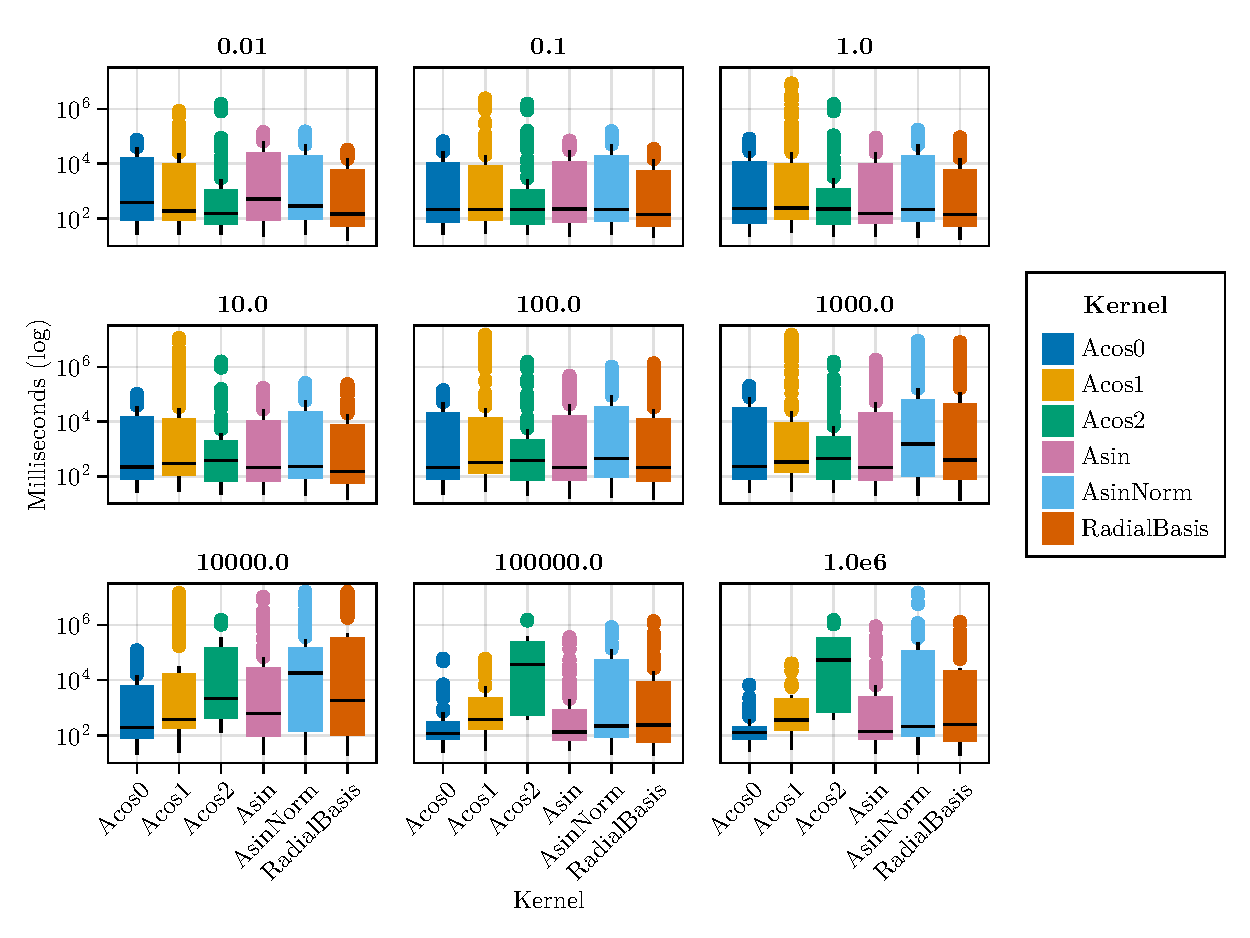
\includegraphics{plots/execution_log}
    \caption{Execution time of the different kernels (log scale) Changing the cost
        parameter}%
    \label{fig:execution-log}
\end{figure}

\Cref{fig:execution-log} shows boxplots of the execution times of the different
kernels for across all datasets. The title above each subplot indicates the
value of the cost parameter. As we can see, increasing the cost parameter
increases the execution time of the SVM. This effect is more noticeable for the
kernels with more complex computations, such as the normalized arc-sine kernel
and specially the arc-cosine kernels with $n=1$ and $n=2$.

\begin{cnote}
    These values of the cost are too high.
    In the other plots, we use $10^4$ as the upper bound.
    We should probably remove the bottom row altogether.

    Also, add cost=... to the subplot titles
\end{cnote}

\begin{figure}[H]
    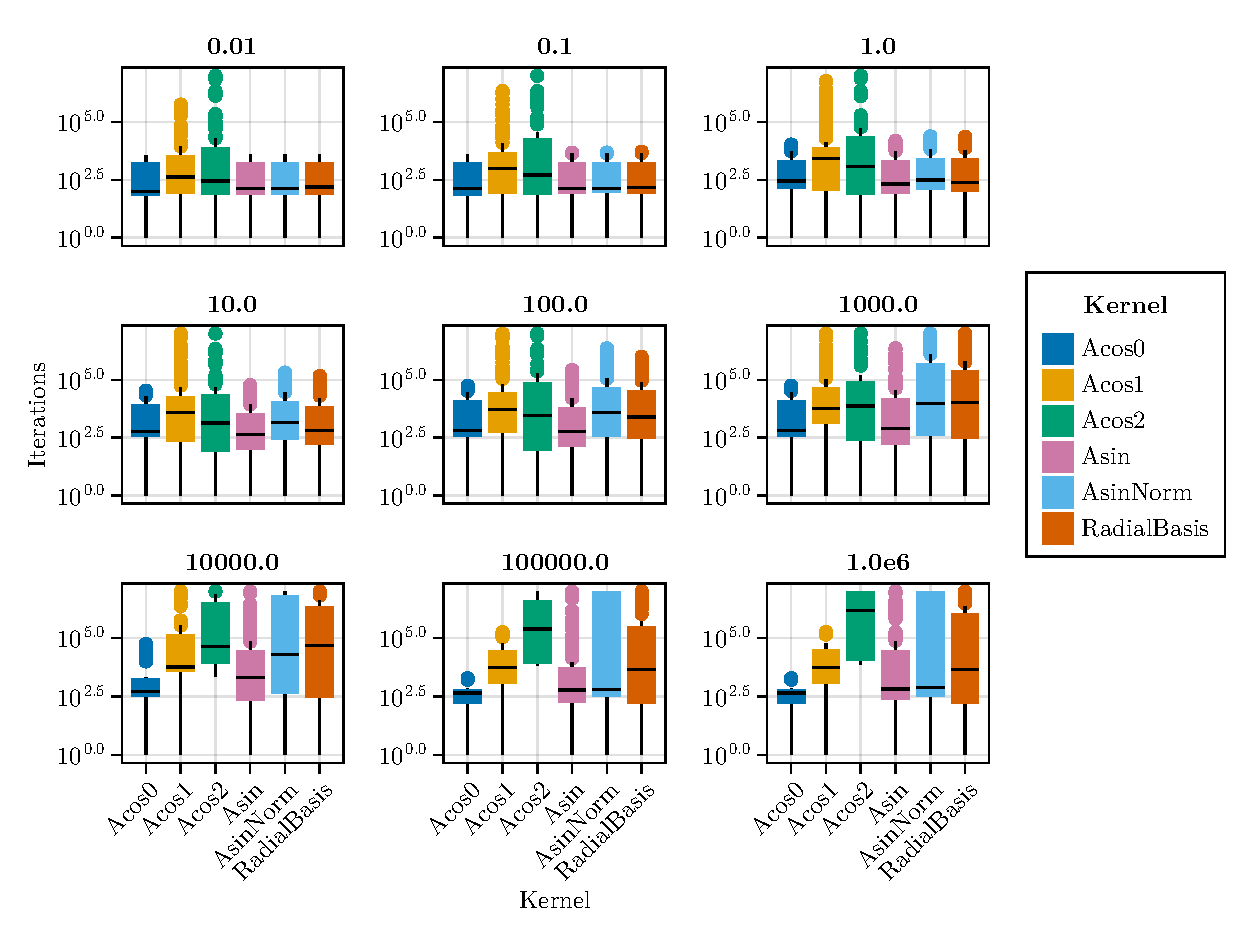
\includegraphics{plots/iter_log}
    \caption{Iterations needed for different kernels (log scale) Changing the cost
        parameter}
\end{figure}

\begin{cnote}
    Why asin-norm has more iterations than asin in average?
\end{cnote}

\section{Comparing the performance of the kernels with different datasets}%
\sectionmark{Comparing performance}

\subsection{Delve (Bank and PumaDyn) dataset families}

The Delve datasets are a collection of datasets used in the Delve project,
among them are the Bank and PumaDyn datasets. There are 8 variations of
these datasets, which come from the combination of these properties%
\footnote{\url{https://www.cs.toronto.edu/~delve/data/families.html}}:
\begin{description}
    \item[Attributes] 32 or 8
    \item[Linearity] Fairly linear or Nonlinear
    \item[Noise] High or Low.
\end{description}

% We refer to a specific combination as \texttt{Bank32fh}, which corresponds to
% the Bank dataset with 32 attributes, \textbf{f}airly linear and \textbf{h}igh
% noise.

\subsubsection{Bank}

\begin{figure}[H]
    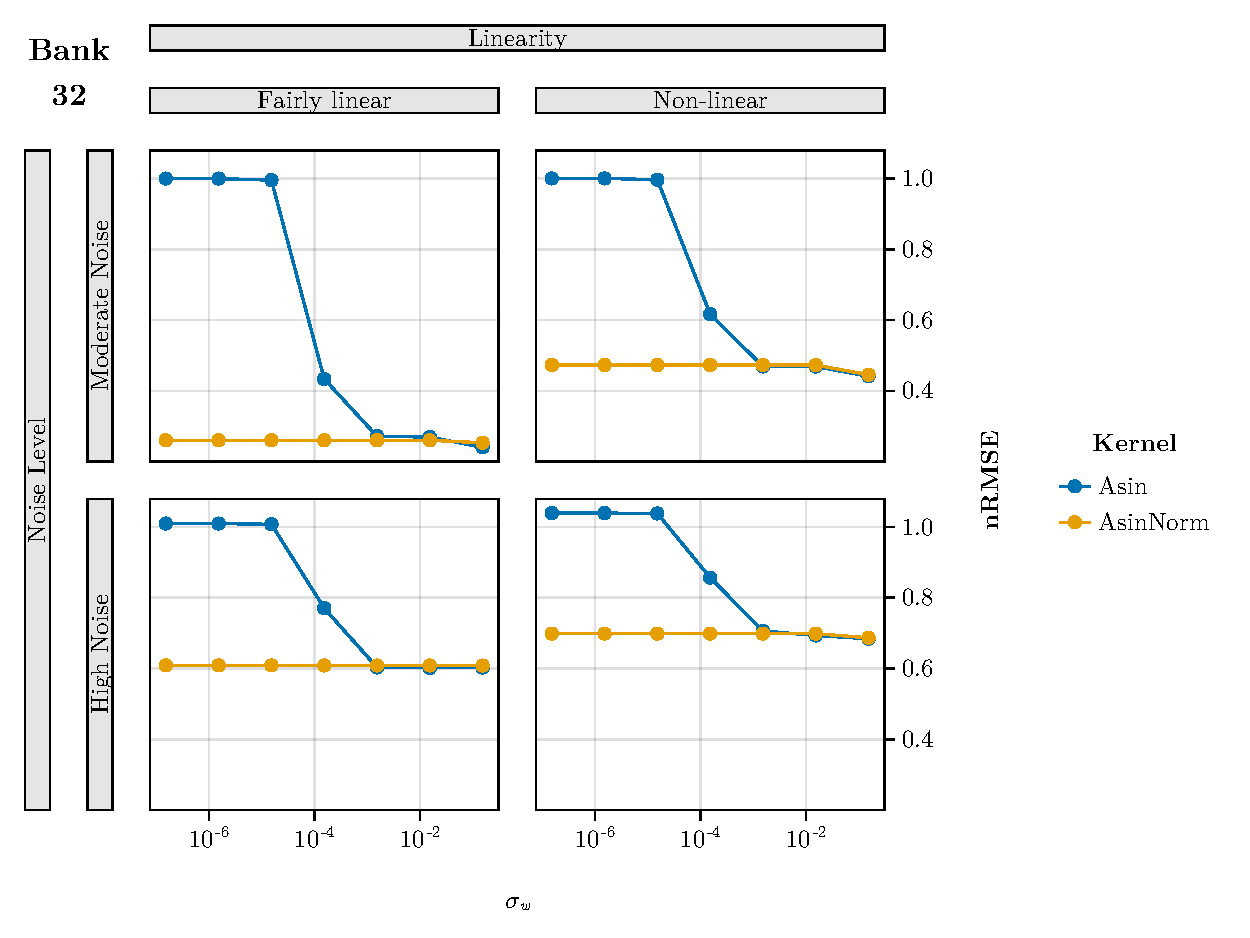
\includegraphics[width=0.7\textwidth]{plots/nRMSE_delve_bank_32_scaled}
    \caption{nRMSE results on Delve Bank32 dataset with $\sigma_w$ scaled}
    \label{fig:nrmse-delve-bank-32-scaled}
\end{figure}

\begin{figure}[H]
    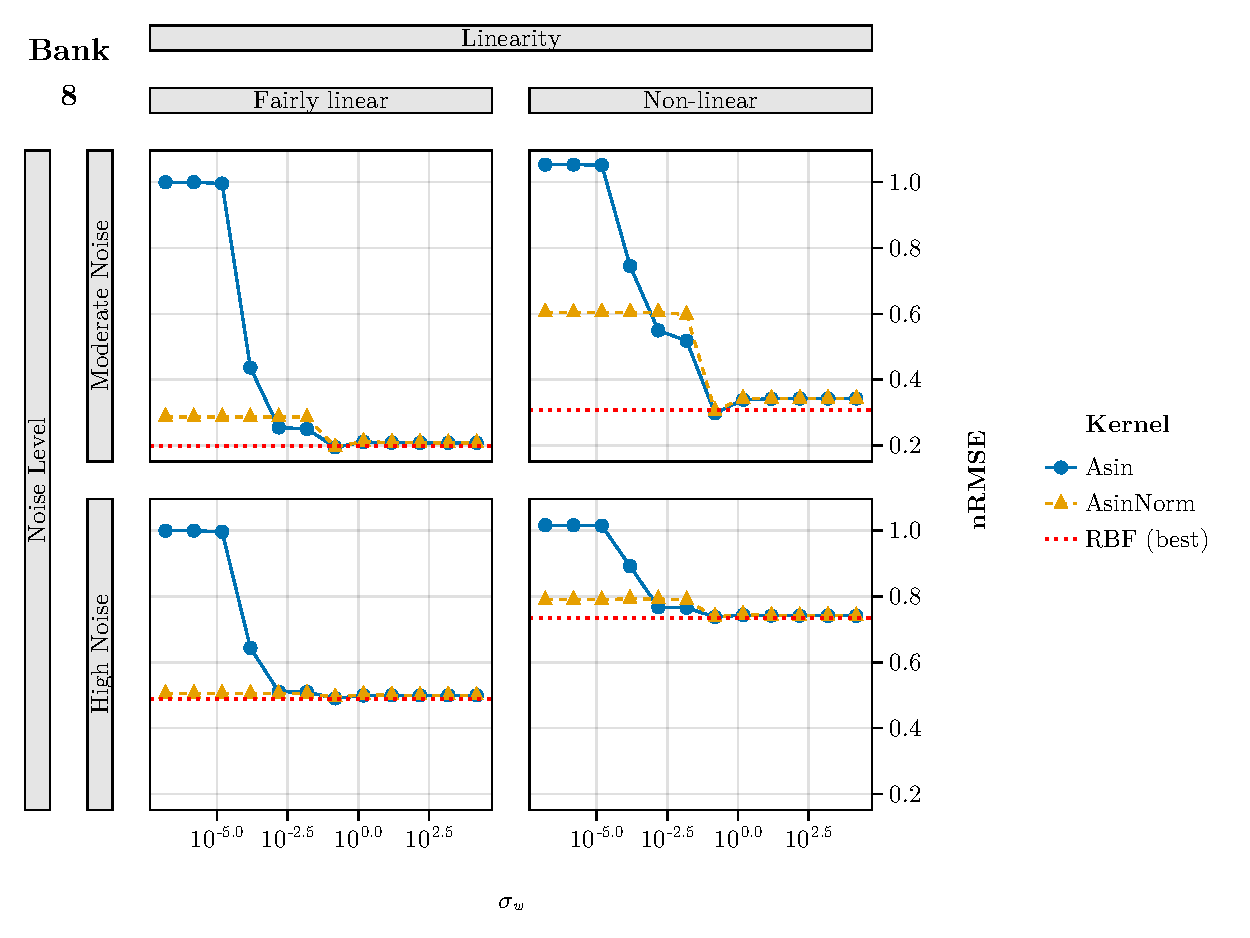
\includegraphics[width=0.7\textwidth]{plots/nRMSE_delve_bank_8_scaled}
    \caption{nRMSE results on Delve Bank8 dataset with $\sigma_w$ scaled}
    \label{fig:nrmse-delve-bank-8-scaled}
\end{figure}

\subsubsection{Pumadyn}

\begin{figure}[H]
    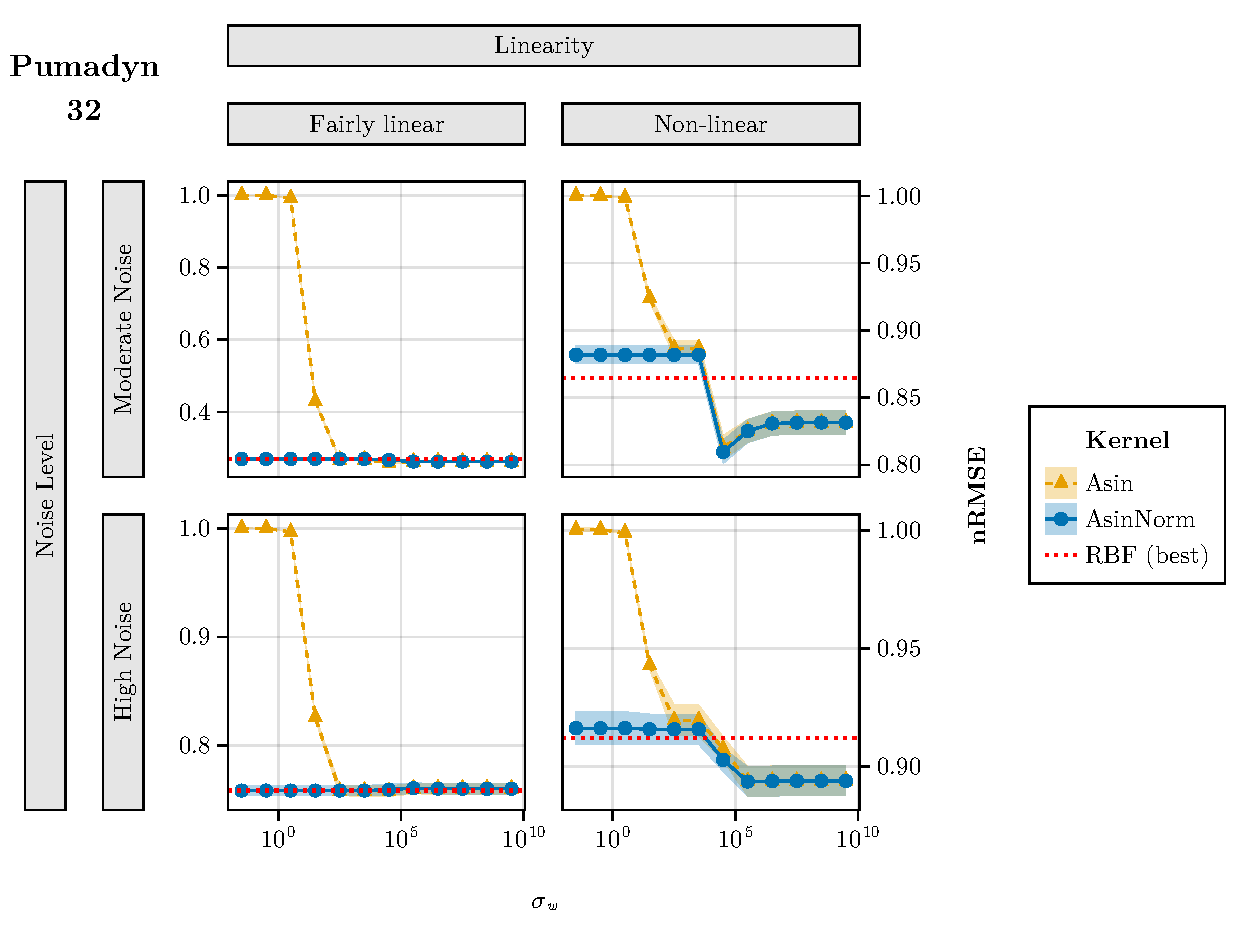
\includegraphics[width=0.7\textwidth]{plots/nRMSE_delve_pumadyn_32_scaled}
    \caption{nRMSE results on Delve PumaDyn32 dataset with $\sigma_w$ scaled}
    \label{fig:nrmse-delve-pumadyn-32-scaled}
\end{figure}

\begin{figure}[H]
    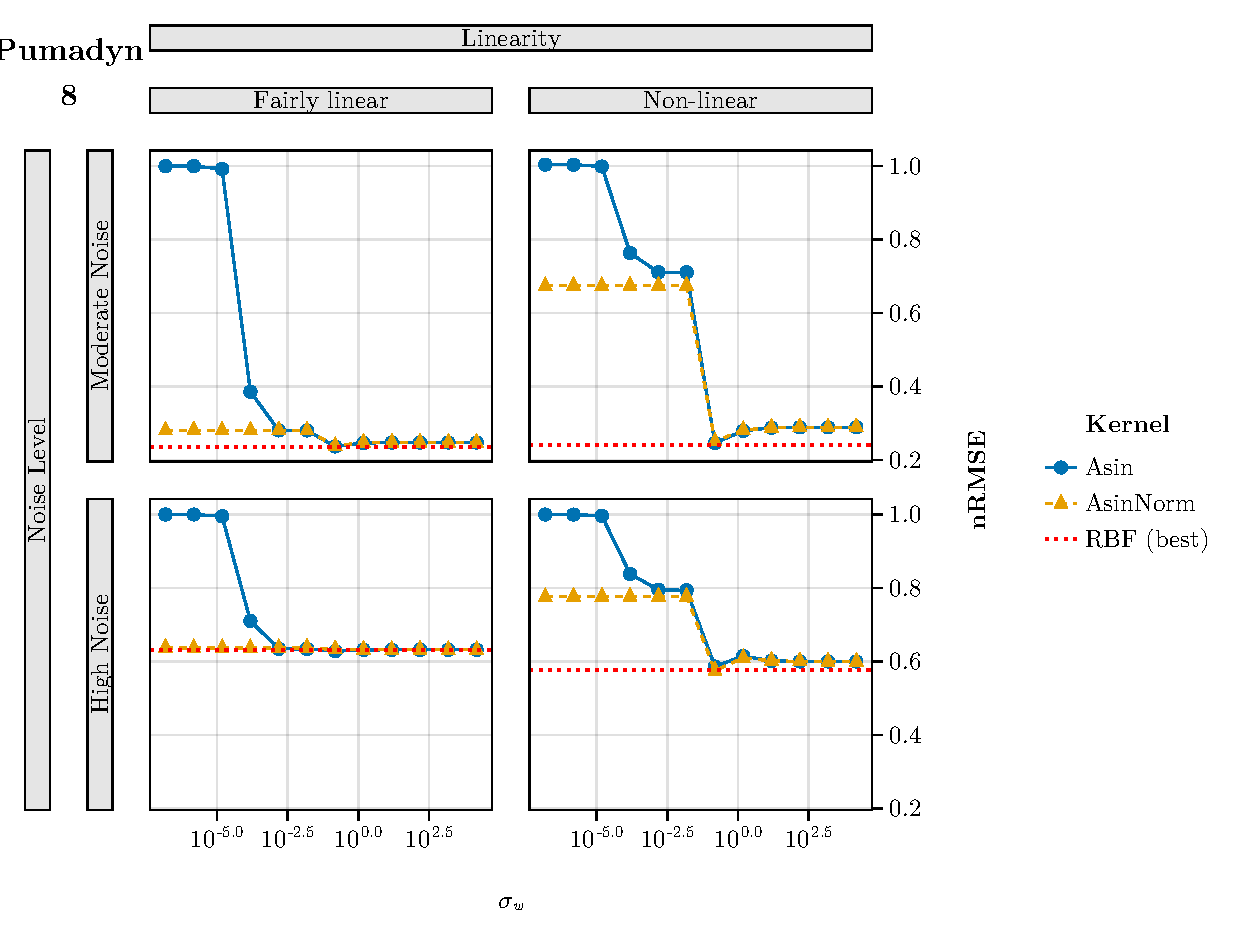
\includegraphics[width=0.7\textwidth]{plots/nRMSE_delve_pumadyn_8_scaled}
    \caption{nRMSE results on Delve PumaDyn8 dataset with $\sigma_w$ scaled}
    \label{fig:nrmse-delve-pumadyn-8-scaled}
\end{figure}

\Cref{fig:nrmse-delve-bank-32-scaled,fig:nrmse-delve-bank-8-scaled,fig:nrmse-delve-pumadyn-32-scaled,fig:nrmse-delve-pumadyn-8-scaled}
show the results obtained on the different datasets in the Band and PumaDyn
families. We can see that the arc-sine kernels do converge when $\sigma_w > 1$.
In the fairly linear datasets, there is not much difference to the RBF kernel,
but in the non-linear there are situations where there is a noticeable
difference. In particular, we see a similar behaviour to the one observed in the
CPU dataset, in which there is a value of $\sigma_w$ that is \emph{optimal} (in
the sense that is not significantly different from the RBF kernel) but
increasing $\sigma_w$ does worsen the performance. This seems to contradict the
theory that there is a threshold $t$ for which increasing $\sigma_w > t$ does
not affect the result and this result is optimal.

It seems that the linearity of the dataset determines whether the arc-sine
kernel performs as the state-of-the-art RBF kernel or not when $\sigma_w$ is
large. This is an interesting result, since we may be able to use meta-learning
to determine if a dataset is a good candidate for the arc-sine kernel or not.

% TODO: can we really draw conclusions from this?

\subsection{Delve (Bank and PumaDyn) dataset using arc cosine}

% TODO: every result with acos is weird

\subsubsection{Bank}

\begin{figure}[H]
    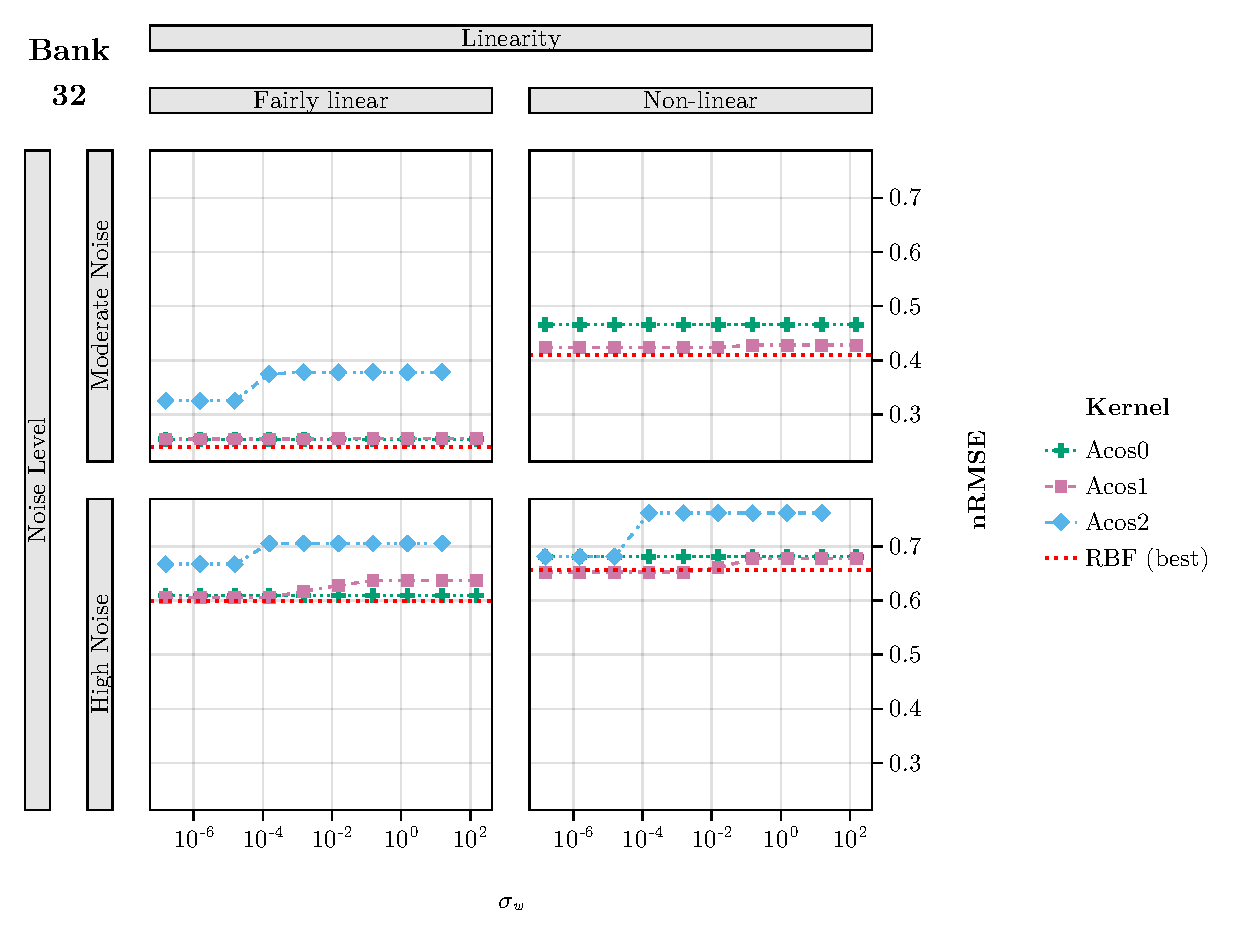
\includegraphics[width=0.7\textwidth]{plots/nRMSE_acos_delve_bank_32_scaled}
    \caption{nRMSE results on Delve Bank32 dataset with $\sigma_w$ scaled}
    \label{fig:nrmse-acos-delve-bank-32-scaled}
\end{figure}

\begin{figure}[H]
    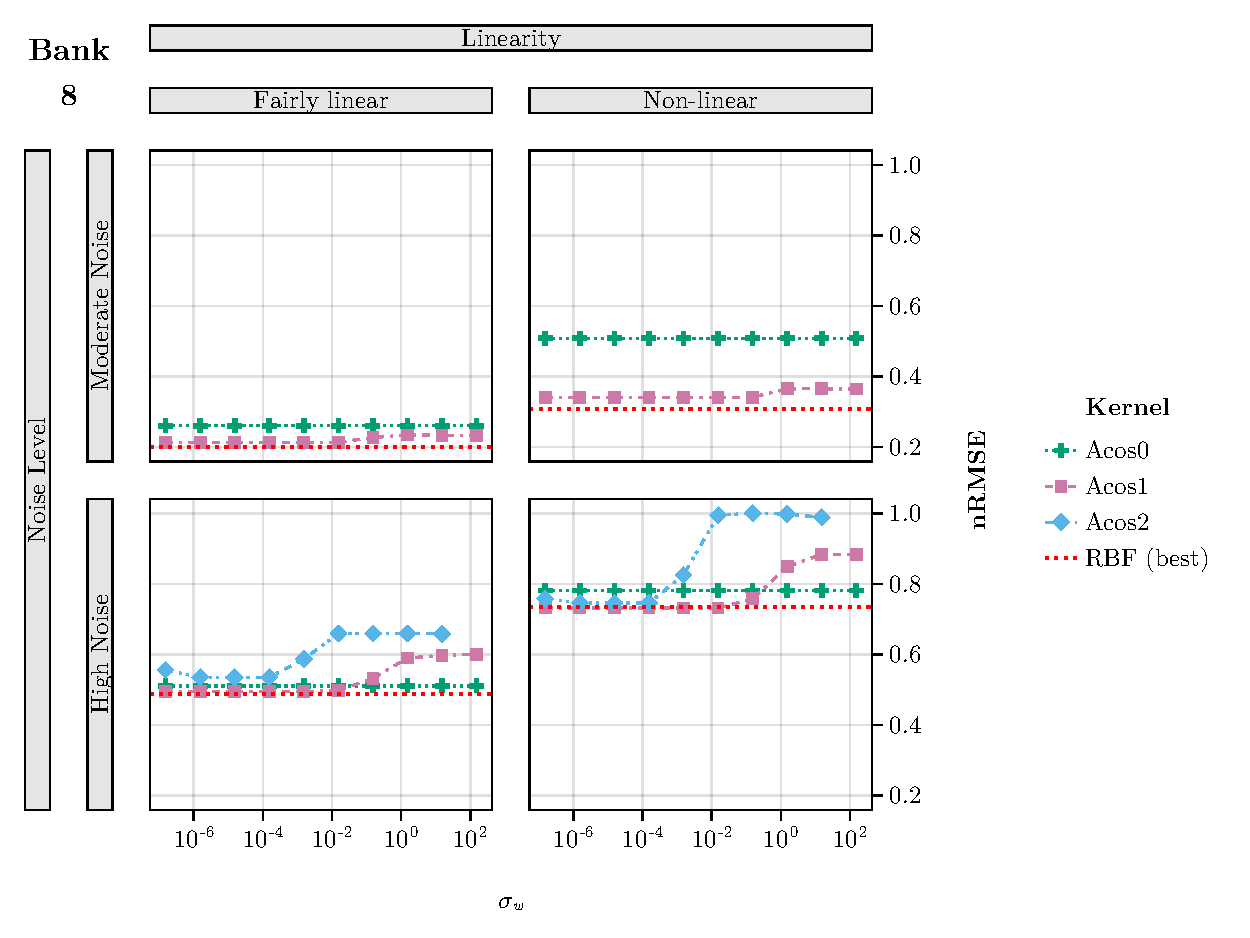
\includegraphics[width=0.7\textwidth]{plots/nRMSE_acos_delve_bank_8_scaled}
    \caption{nRMSE results on Delve Bank8 dataset with $\sigma_w$ scaled}
    \label{fig:nrmse-acos-delve-bank-8-scaled}
\end{figure}

\subsubsection{Pumadyn}

\begin{figure}[H]
    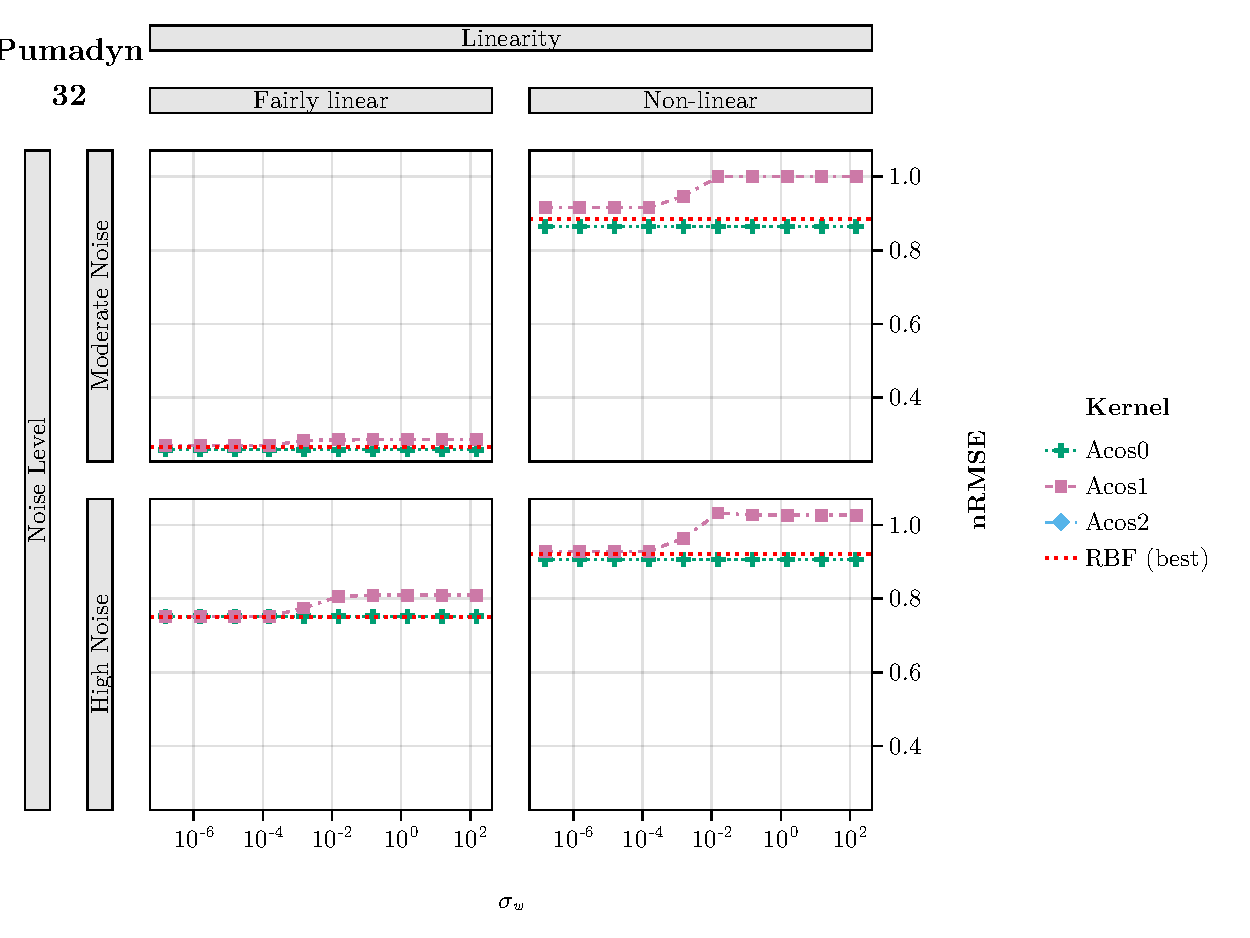
\includegraphics[width=0.7\textwidth]{plots/nRMSE_acos_delve_pumadyn_32_scaled}
    \caption{nRMSE results on Delve PumaDyn32 dataset with $\sigma_w$ scaled}
    \label{fig:nrmse-acos-delve-pumadyn-32-scaled}
\end{figure}

\begin{figure}[H]
    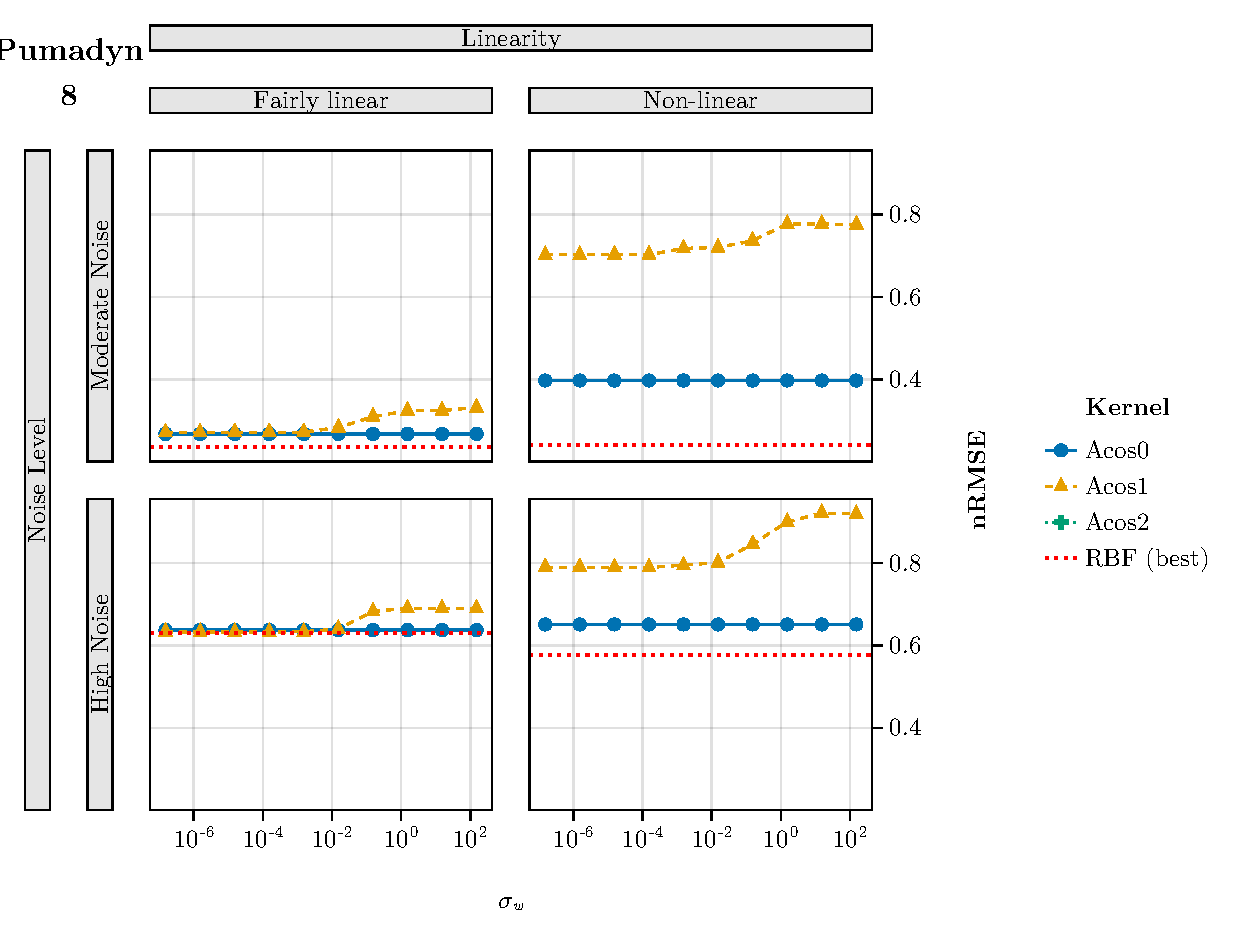
\includegraphics[width=0.7\textwidth]{plots/nRMSE_acos_delve_pumadyn_8_scaled}
    \caption{nRMSE results on Delve PumaDyn8 dataset with $\sigma_w$ scaled}
    \label{fig:nrmse-acos-delve-pumadyn-8-scaled}
\end{figure}

\begin{figure}[H]
    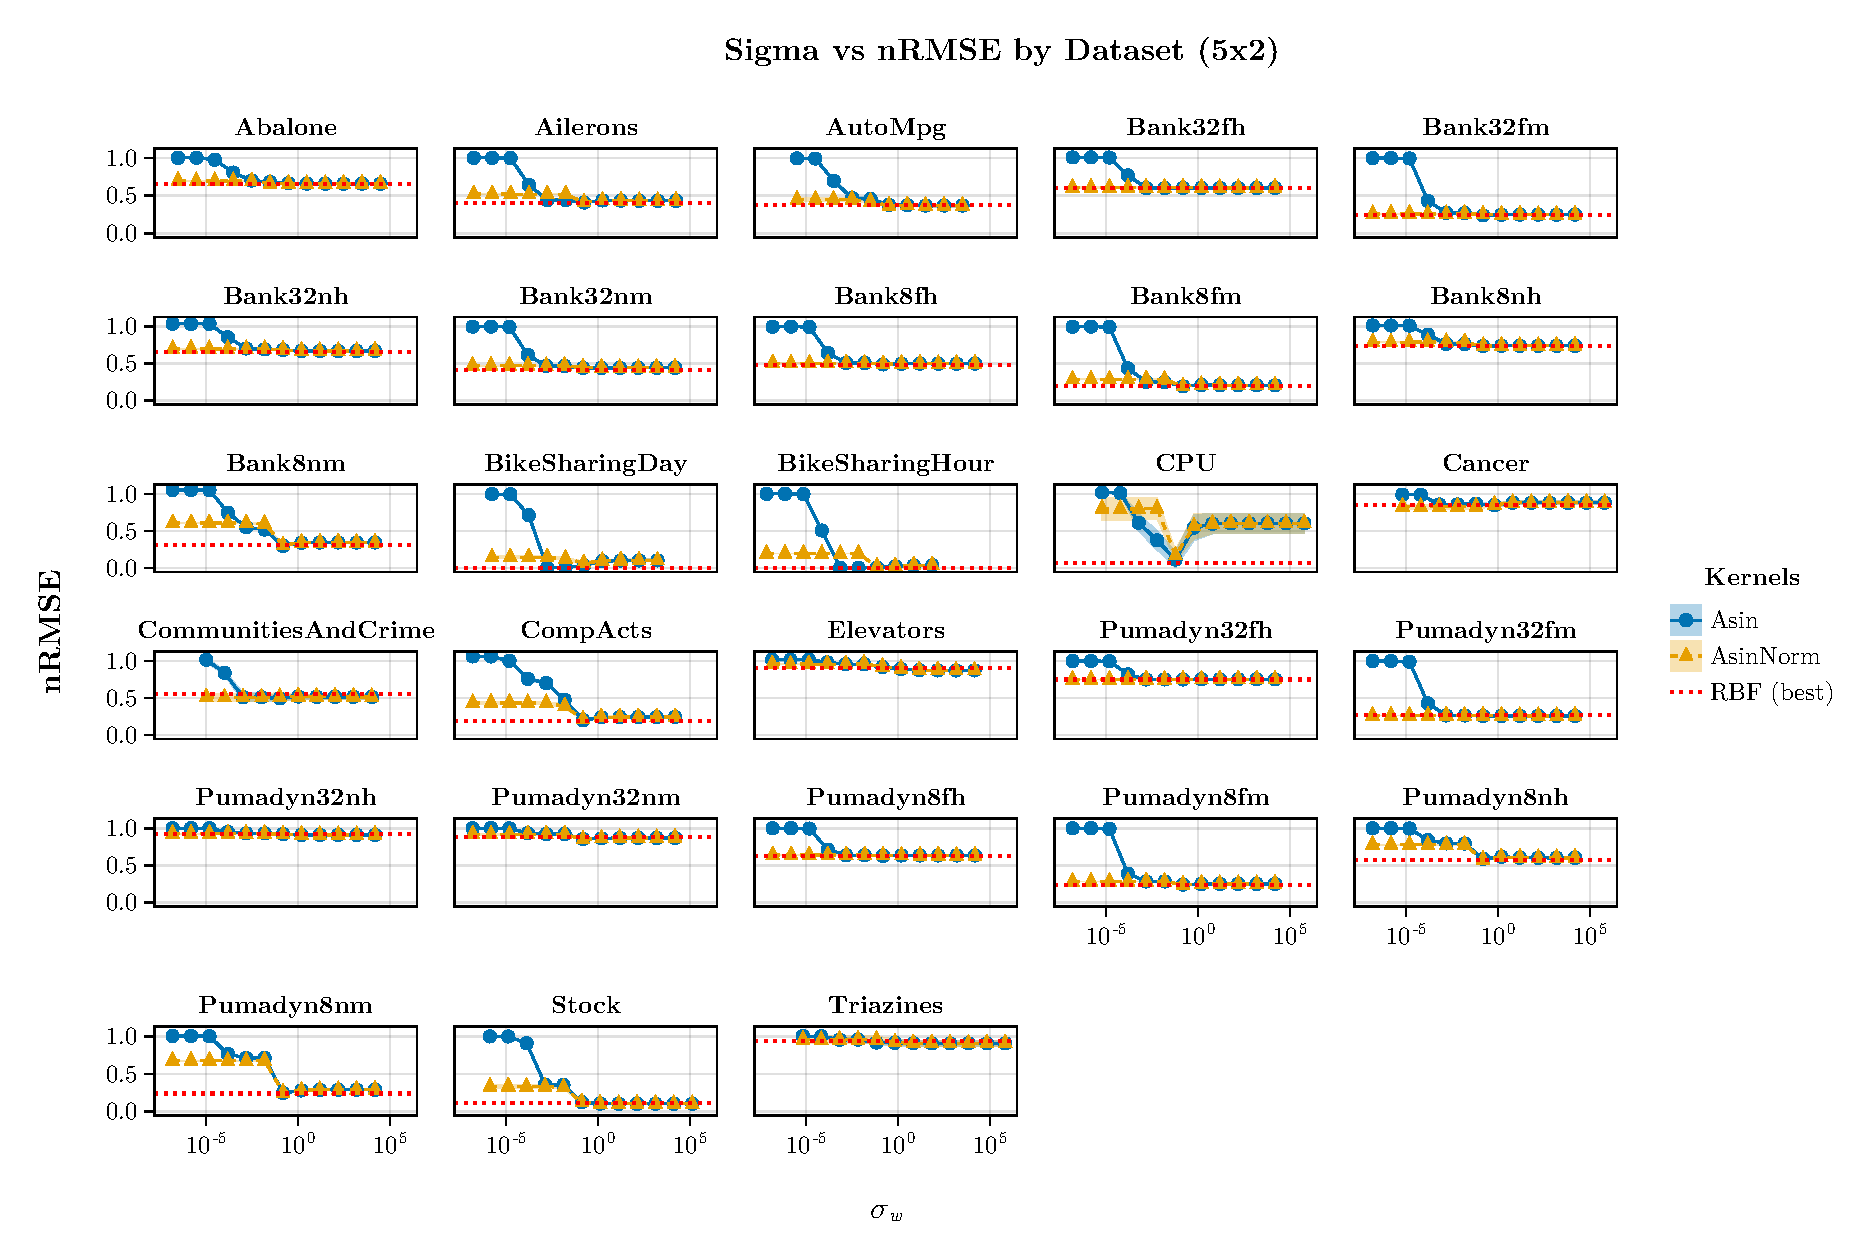
\includegraphics[width=0.9\textwidth]{plots/nRMSE_all_scaled}
    \caption{nRMSE results on all datasets with $\sigma_w$ scaled}
    \label{fig:nrmse-all-scaled}
\end{figure}


